
\documentclass[11pt]{exam} % https://www.ctan.org/pkg/exam?lang=en

\usepackage[lmargin=1.in,rmargin=1.in,tmargin=1.in,bmargin=1in]{geometry}
\usepackage{setspace}
\usepackage[pdftex]{graphicx}
\usepackage{titling}
\usepackage[
	pdfauthor={Brian Weinstein},
	pdftitle={Homework 3},
	bookmarks=true,
	colorlinks=true,
	linkcolor=blue,
	urlcolor=blue,
	citecolor=blue,
	pdftex,
	linktocpage=true
	]{hyperref}
\usepackage[textsize=tiny]{todonotes}
\usepackage{float}
\setlength\parindent{0pt}
\usepackage{lipsum}


\qformat{\textbf{Problem \thequestion: \thequestiontitle}\quad \hfill}


\pagestyle{headandfoot}
\runningheadrule
\firstpageheader{}{}{}
\runningheader{\thetitle}{\theauthor}{\thedate}
\firstpagefooter{}{\thepage}{}
\runningfooter{}{\thepage}{}


\usepackage{xcolor}
\usepackage{adjustbox}
\usepackage{verbatim}
\definecolor{shadecolor}{rgb}{.9, .9, .9}

\newenvironment{code}%
   {\par\noindent\adjustbox{margin=1ex,bgcolor=shadecolor,margin=0ex \medskipamount}\bgroup\minipage\linewidth\verbatim}%
   {\endverbatim\endminipage\egroup}

\newenvironment{codeSmall}%
   {\par\noindent\adjustbox{margin=1ex,bgcolor=shadecolor,margin=0ex \medskipamount}\bgroup\minipage\linewidth\verbatim\footnotesize}%
   {\endverbatim\endminipage\egroup}





\begin{document}


\title{STAT S4240 002, Homework 3}
\author{Brian Weinstein (bmw2148)}
\date{July 30, 2015}
\maketitle



\begin{questions}



\titledquestion{question name}

\begin{parts}



\part asdf asdf asdf
\begin{code}
> apply(rawData, 2, mean)
       x1        x2        x3        x4        x5 
 6.049104 -8.277221  4.665532  7.914270 62.138753 
\end{code}
 
\part ASDF ASDF ASDF
\begin{codeSmall}
> apply(rawData, 1, mean)
  [1]  -0.1277116  20.8162864  -8.8984358  25.5999204  -9.7472153
  [6]  64.0626702  22.0392371  23.3914888  31.7598224 -13.8680290
...
 [91]   1.2105932  21.2145724  -8.4896595  19.0639963  20.9767512
 [96]   3.5962333  22.3461063   0.7145014   6.3080005  64.8829556
\end{codeSmall}

 
 
%\begin{figure}[H]
%	\centering
%	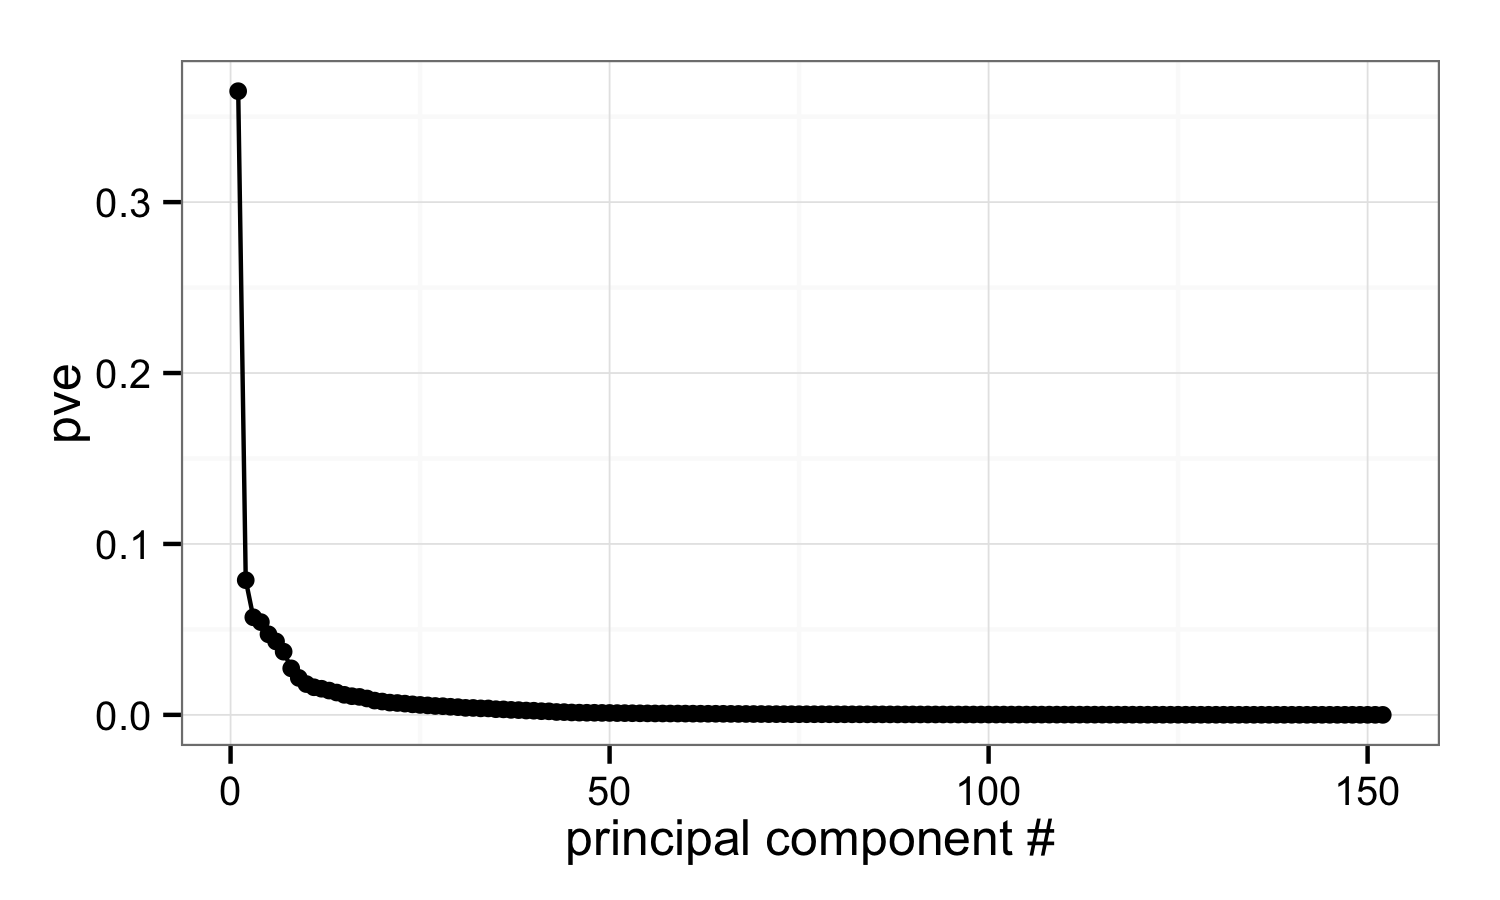
\includegraphics[width=5in]{2c.png}
%	%\caption{}
%	%\label{fig:figName}
%\end{figure}


\end{parts}



\titledquestion{question name 2}

\begin{parts}

\part \lipsum[3-5]


\end{parts}





\end{questions}

%\listoftodos

\end{document}